\documentclass[11pt]{article}

\usepackage{fullpage}
\usepackage{graphicx}
\begin{document}

\title{ARM Checkpoint... }
\author{Istvan Darok, James Shipley, Prashant Gurung}

\maketitle

\section{Group Organisation}

A lot of improvement could be made to how we split up the work between group members, as we
struggled to effectively allocate tasks evenly between everyone. The work on the project started
late due to lack of communication, but once we started we managed to get everyone to the same
level of profiency in C fairly quicky by making a progress table. This level of organisation 
deteriorated once we started to code towards a solution. This was partially due to a failure to 
decompose the problem, which lead to members being left without work to do in the first two days.
Another contributing factor to the breakdown of our organisation was one team member assigned to
our group left the course, and dropped out of the project on the first day of coding.
\\~\\On the first day (Monday), James and Prashant focused on the development of the loader, while Istvan and Graham
developed pseduocode for the structure of the emulator. We had a meeting at the start of the day
to develop a plan of action for the team but we did not hold one at the end of the day to check our progress.
\\~\\On the second day (Tuesday), we had a meeting where we finalised the structure of our emulator implementation.
James finished the loader and finished work on the decoder, while Prashant and Istvan 
started work on execute\_dp separately.
\\~\\On the third day (Wednesday), James completed execute\_sdt and focused on making changes to the data structures of the emulator,
Istvan started work on execute\_m and Prashant finished execute\_dp.
\\~\\On the fourth day (Thursday), we started to assemble the independent functions we had made together so that it works seamlessly 
as one code. We also began testing our functions and checking the register outputs. We also refactored
the code to make it more concise.
\\~\\On the last day (Friday), we completed the report and did further testing.
\\~\\The main strengths of the team were that we managed to define a complete structure for the emulator
early on in the project development. This allowed us to base all of our codes on that specific structure,
and no work was needed to ensure that all functions were compatible with each other.
\\~\\The main changes that we need to make for the later tasks are to start using the git repository so
that we can efficiently share code with each other, and so our code structure would be more organised.
Our orignial method of using Microsoft Teams to share code is not scalable and is not considered a good
practice. We should also allocate more time to pair programming sessions and do more live coding during
meetings.
\section{Implementation Strategies}
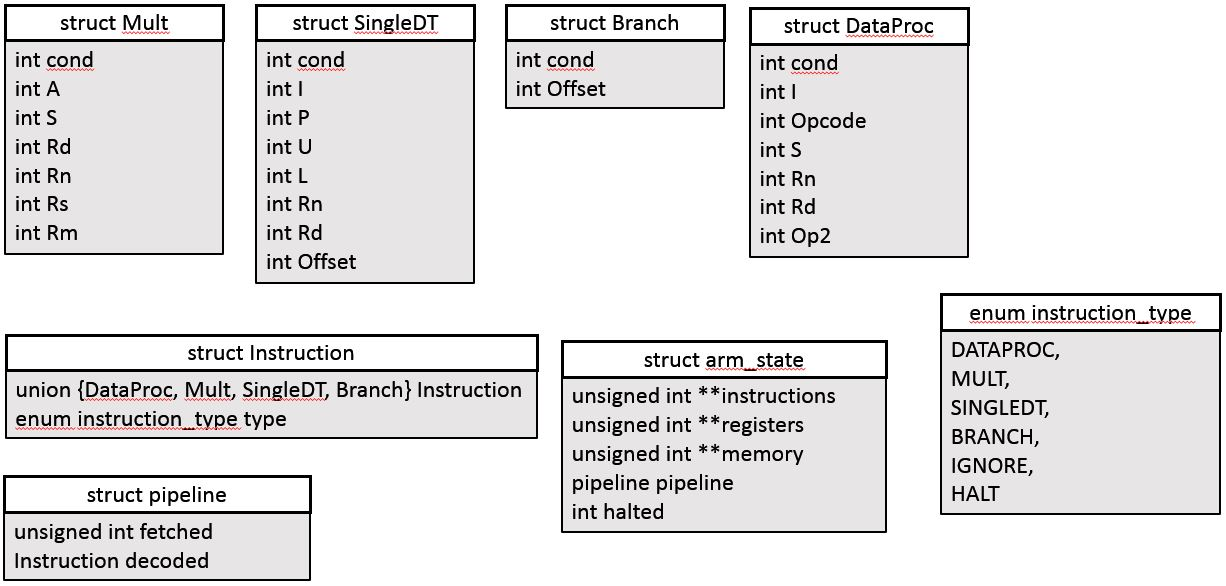
\includegraphics[width=12cm]{Capture.JPG}
\\~\\
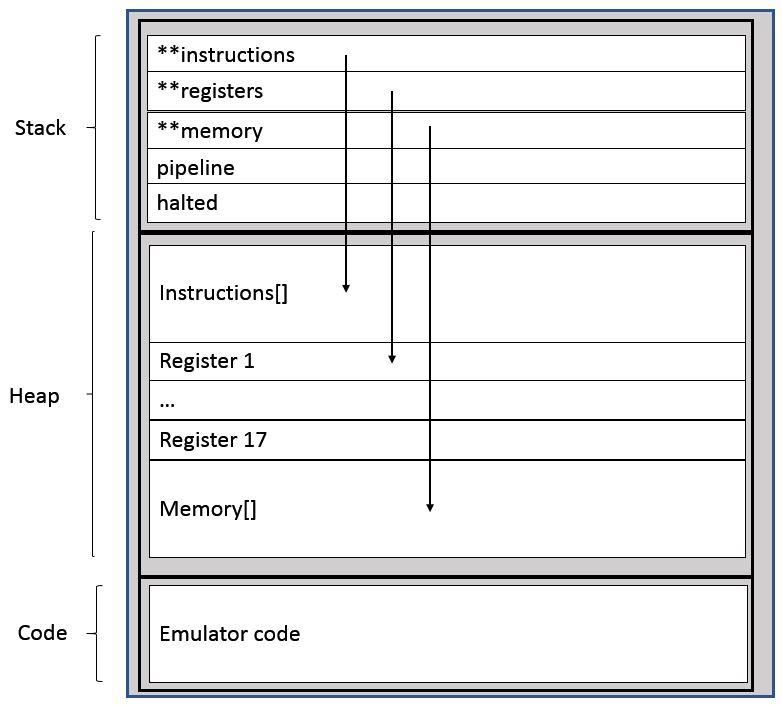
\includegraphics[width=12cm]{sasd.JPG}
\\~\\
An instruciton consists of 4 instruction types. It can be either Data Processing, Multiply, Single Data Transfer, or Branch.
Thus we thought it would be a good idea to represent these type as a  struct. This allows us to reference important sections
of different instructions with ease. Since an instruction can only be one instruction type, we thought it would be a good idea to
use a union to capture this idea and pair it with an enum which tells us the instruction type it is holding.
\\The pipeline struct represents the pipeline at any stage of execution, just like figure 1 in the spec.
\\~\\
The arm\_state struct is the main structure that we use to represent the arm11 machine. it contains pointers to all of the relevant arrays,
as well as the pipeline, and a variable to represent whether the machine has halted. This is the main structure that is passed through
each function, and allows the registers and memory to be accessed and changed easily by the revelant functions.
\\~\\
We will reuse the data structure and the loader that we have previously defined, though the loader might 
need to be updated to accommodate for the different data format. We might use auxiliary functions such as
getBits and modifyBits, however the decode and execute functions are not particularly applicable in the context to
the assembler algorithm.
\\~\\The main tasks that we will find challenging are the extension and the implementing the data processing
algorithm for the assembler. We are attempting to mitigate these issues by researching various extension project, and
closely reading the spec for the assembler. 

\end{document}
